%
% 41-beispiel.tex -- Ein einführendes Beispiel
%
% (c) 2026 Prof Dr Andreas Müller
%
\subsection{Ein einführendes Beispiel
\label{buch:integration:residuen:section:beispiel}}
%
% cauchy-verteilung.tex
%
% (c) 2026 Prof Dr Andreas Müller
%
\begin{figure}
\centering
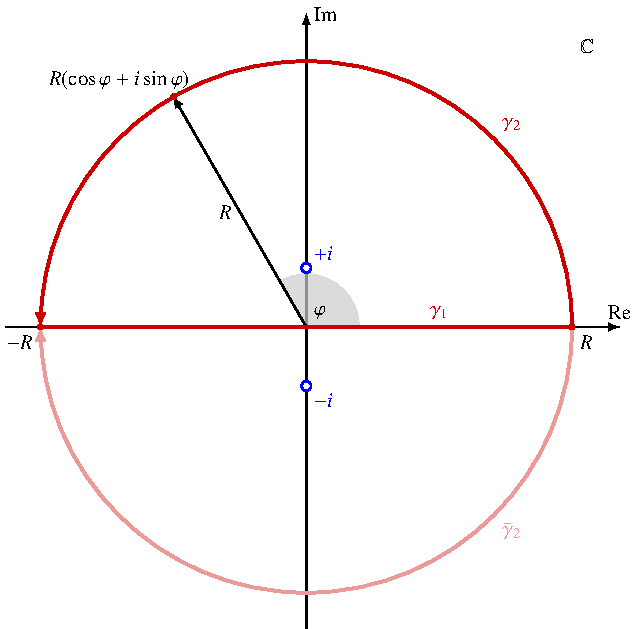
\includegraphics{chapters/030-integration/images/cauchyverteilung.pdf}
\caption{Integrationsweg für die Berechnung der Integrale
\eqref{buch:integration:residuen:eqn:cauchyintegral}
und
\eqref{buch:integration:residuen:eqn:ecos}.
\label{buch:integration:residuen:fig:cauchyverteilung}}
\end{figure}
%
Als einführendes Beispiel betrachten wir die Berechnung des uneigentlichen
Integrals
\index{uneigentliches Integral}%
\index{Integral!uneigentlich}%
\begin{equation}
I
=
\int_{-\infty}^\infty \frac{1}{x^2+1} \,dx.
\label{buch:integration:residuen:eqn:cauchyintegral}
\end{equation}
Es tritt zum Beispiel auf bei der Berechnung der Normierungskonstanten
der Cauchy-Verteilung, die die Wahrscheinlichkeitsdichte
\[
\varphi(x)
=
\frac{1}{\pi\gamma
\biggl(
\displaystyle
1+\biggl(\frac{x-x_0}{\gamma}\biggr)^2
\biggr)}
\]
hat.
Der Erwartungswert dieser Verteilung ist $x_0$, die Varianz und allere
höheren Momente sind nicht definiert.
\index{Verteilung}%
\index{Erwartungswert}%
Die $t$-Verteilung mit einem Freiheitsgrad ist ein Cauchy-Verteilung.
\index{Cauchy-Verteilung}%
\index{Verteilung!Cauchy-}%

%
% Berechnung mit der Stammfunktion
%
\subsubsection{Berechnung mit der Stammfunktion}
Zur Berechnung des
Integrals~\eqref{buch:integration:residuen:eqn:cauchyintegral}
kann natürlich die Stammfunktion verwendet werden, die in diesem
Fall einfach zu berechnen ist.
Es gilt nämlich
\[
\frac{d}{dx}\arctan(x)
=
\frac{1}{x^2 + 1}.
\]
Daher ist das Integral
\[
\int_a^a
\frac{1}{x^2+1}
\,dx
=
\Bigl[
\arctan(x)
\Bigr]_{-a}^a
=
\arctan(a) - \arctan(-a).
\]
Für das
Integral~\eqref{buch:integration:residuen:eqn:cauchyintegral}
muss der Grenzwert $a\to\infty$ berechnet werden, der
\[
\int_{-\infty}^\infty \frac{1}{x^2+1} \,dx
=
\lim_{a\to\infty}
\bigl(
\arctan(a) -\arctan(-a)
\bigr)
=
\lim_{a\to\infty} 2\arctan(a)
=
2\cdot\frac{\pi}2
=
\pi
\]
ist.

%
% Berechnung mit einem Wegintegral
%
\subsubsection{Berechnung mit einem Wegintegral}
Die Funktion
\[
z
\mapsto
f(z)
=
\frac{1}{z^2 + 1}
=
\frac1{2i}
\biggl(
\frac{1}{z-i}
-
\frac{1}{z+i}
\biggr)
\]
ist ganz offensichtlich eine holomorphe Funktion, die überall in der
komplexen Ebene ausser in den Punkten $\pm i$ definiert ist.

Ein Wegintegral entlang eines Weges, der den Punkt $+i$ umläuft,
aber nicht den Punkt $-i$,
hat den Wert
\begin{align*}
\oint_\gamma f(z)\,dz
&=
\frac1{2i}
\oint_\gamma \frac{1}{z-i}
\,dz
-
\frac1{2i}
\oint_\gamma \frac{1}{z+i}
\,dz.
\intertext{Da die Kurve den Punkt $-i$ nicht umläuft, verschwindet
das zweite Integral.
Das erste Integral kann
durch ein Integral eines 
kleinen Kreises mit der Parameterdarstellung $\gamma(t)=i+r e^{2\pi it}$
um den Punkt $+i$ ersetzt werden und ergibt}
&=
\frac{1}{2i}
\int_0^1
\frac{1}{(i+e^{2\pi it})-i}
2\pi i e^{2\pi it}\,dt
\\
&=
\frac{1}{2i}
\cdot
2\pi i
\int_0^1 
\,dt
=
\pi.
\end{align*}

Das
Integral~\eqref{buch:integration:residuen:eqn:cauchyintegral}
muss jetzt mit einem konkret gewählten Weg berechnet werden.
Dazu wählen wir den in
Abbildung~\ref{buch:integration:residuen:fig:cauchyverteilung}
dargestellten Weg.
Er führt erst als $\gamma_1$ der $x$-Achse entlang von $-R$ bis
zum Punkt $R$ und dann als $\gamma_2$ in einem grossen Halbkreis
vom Radius $R$ um den Nullpunkt wieder zurück zu $-R$.
Als Parametrisierungen für diese Wege kann man
\[
\begin{aligned}
\gamma_1(x)
&=x&
&\qquad&
&\text{für $-R\le x \le R$},
\\
\gamma_2(\varphi)
&=Re^{i\varphi}=R(\cos\varphi+i\sin\varphi)&
&\qquad&
&\text{für $0\le \varphi\le \pi$}
\end{aligned}
\]
verwenden.
Das Integral über diesen Pfad setzt sich zusammen aus den Integralen
über die beiden Teilpfade:
\begin{equation}
\begin{aligned}
\pi
=
\oint_\gamma f(z)\,dz
&=
\int_{\gamma_1} f(z)\,dz
+
\int_{\gamma_2} f(z)\,dz
\\
&=
\int_{-R}^R \frac{1}{z^2+1} \,dz
+
\int_0^{\pi} \frac{1}{R^2e^{2i\varphi}+1}\cdot iRe^{i\varphi}\,d\varphi.
\end{aligned}
\label{buch:integration:residuen:beispiel:eqn:cauchypfade}
\end{equation}
Das erste Integral konvergiert für $R\to\infty$ gegen das gesuchte
Integral~\eqref{buch:integration:residuen:eqn:cauchyintegral},
es ist also nur noch zu überlegen, was der Grenzwert des zweiten
Integrals für $R\to\infty$ ist.

Wegen
\[
\biggl|
\frac{1}{R^2e^{2i\varphi}+1}
\biggr|
=
\frac{1}{|R^2e^{2i\varphi}+1|}
\le
\frac{1}{R^2-1}
\]
folgt
\begin{align*}
\int_0^{\pi}
\frac{1}{R^2e^{2i\varphi}+1}\cdot iRe^{i\varphi}
\,d\varphi
&\le
\int_0^{\pi}
\frac{R}{R^2-1}
\,d\varphi
=
\frac{\pi R}{R^2-1}.
\end{align*}
Der Grenzwert auf der rechten Seite für $R\to\infty$ ist $0$, das
Integral über $\gamma_2$ trägt also nichts bei.
Somit folgt
\[
\pi 
=
\int_{-\infty}^\infty \frac{1}{x^2+1}\,dx,
\]
das selbe Resultat, wie wir mit der Stammfunktion gefunden haben.

%
% Ein mit der Stammfunktion nicht lösbares Beispiel
%
\subsubsection{Ein mit der Stammfunktion nicht lösbares Beispiel}
Wir wollen das Integral
\begin{equation}
\int_{-\infty}^\infty
\frac{\cos tx}{x^2+1}
\,dx
\label{buch:integration:residuen:eqn:ecos}
\end{equation}
für $t>0$ berechnen.
Es tritt zum Beispiel bei der Berechnung des Erwartungswertes 
$E(\cos(X))$ einer Cauchy-verteilten Zufallsvariable $X$ auf.
Um es mit der oben skizzierten Methode berechnen zu können,
müssen wir den Integranden erst in eine holomorphe Funktion
umwandeln.
Der Kosinus ist der Realteil $\cos x = \operatorname{Re}e^{itx}$,
auf der reellen Achse gilt also
\[
\frac{\cos x}{x^2+1}
=
\operatorname{Re}\frac{e^{itx}}{x^2+1}
\qquad
\text{für $x\in\mathbb{R}$}.
\]
Zur Berechnung des Integrals~\eqref{buch:integration:residuen:eqn:ecos}
können wir also die holomorphe Funktionen
\begin{equation}
f(z)
=
\frac{e^{itz}}{z^2+1}
\end{equation}
verwenden.

Mit dem gleichen Weg
\eqref{buch:integration:residuen:beispiel:eqn:cauchypfade}
wie vorhin können wir versuchen, das Integral
\begin{align*}
\oint_\gamma
\frac{e^{itz}}{z^2+1}
\,dz
&=
\oint_\gamma
\frac{e^{itz}}{2i}
\biggl(
\frac{1}{z-i}
-
\frac{1}{z+i}
\biggr)
\,dz
=
\oint_\gamma
\frac{e^{itz}}{2i}
\biggl(
\frac{1}{z-i}
\,dz
-
\oint_\gamma
\frac{1}{z+i}
\biggr)
\,dz.
\intertext{mit Hilfe des Integralsatzes zu berechnen.
Der Weg $\gamma$ dreht sich einmal um den Punkt $i$, nicht aber um $-i$.
Es bleibt also nur das erste Integral}
&=
\frac{1}{2i}
\oint_\gamma
\frac{e^{itz}}{z-i}
\,dz
=
\pi\cdot 
\frac{1}{2\pi i}
\oint_\gamma
\frac{e^{itz}}{z-i}
\,dz
\intertext{welches nach dem Integralsatz durch den Wert des Zählers
an der Stelle $z=i$ ersetzt werden kann:}
&=
\pi \cdot e^{it\cdot i}
=
\pi e^{-t}.
\end{align*}
Um zu zeigen, dass dies
der gesuchte Wert des Integrals ist, müssen wir den Weg wieder in
die beiden Teile $\gamma_1$ und $\gamma_2$ zerlegen.
\begin{align*}
\oint_\gamma
\frac{e^{itz}}{z^2+1}
\,dz
&=
\int_{-R}^R
\frac{e^{itx}}{x^2+1}
\,dx
+
\int_0^1
\frac{e^{it\gamma_2(t)}}{\gamma_2(t)^2+1}
\,dt.
\end{align*}
Das erste Integral konvergiert für $R\to\infty$ gegen das gesuchte
Integral, wir müssen also nur noch zeigen, dass das zweite Integral
keinen Beitrag leistet.
Dazu müssen wir den Integranden mit Hilfe der Parametrisierung
\[
\gamma_2(\varphi)=R(\cos\varphi+i\sin\varphi)
\qquad\Rightarrow\qquad
|\gamma_2(\varphi)|
=
R
\]
abschätzen:
\begin{align}
\biggl|\frac{e^{itz}}{z^2+1}\biggr|
&=
\frac{|e^{itz}|}{|z^2+1|}
\le
\frac{|e^{itR(\cos \varphi + i\sin\varphi)}|}{|z|^2+1}
=
\frac{|e^{itR\cos\varphi}|\cdot e^{-tR\sin\varphi}}{R^2+1}
\le
\frac{1}{R^2+1}
\label{buch:integration:residuen:bsp:abschaetzung}
\end{align}
Wie im früheren Beispiel folgt
\begin{align*}
\biggl|
\int_{\gamma_2} \frac{e^{itz}}{z^2+1}\,dz
\biggr|
&=
\biggl|
\int_{\gamma_2}
\frac{e^{it\gamma_2(\varphi)}}{\gamma_2(\varphi)^2+1}
\dot\gamma_2(\varphi)
\,d\varphi
\biggr|
\le
\int_0^\pi \frac{1}{R^2+1} R \,dt
=
\frac{\pi R}{R^2+1}.
\end{align*}
Die rechte Seite konvergiert für $R\to\infty$ gegen $0$ und es folgt
\begin{equation}
\int_{-\infty}^\infty
\frac{\cos xt}{x^2+1}
\,dx
=
\operatorname{Re}
\oint_\gamma \frac{e^{itz}}{z^2+1}\,dz
=
\pi e^{-t}
\qquad
\text{für $t\ge 0$}.
\label{buch:integration:residuen:eqn:pie-t}
\end{equation}
Damit ist das Integral berechnet.
Man beachte, dass für diesen Integranden keine Stammfunktion
gefunden werden kann, die vorgestellte Methode ist also die einzige
Methode zur Berechnung des Integrals.

Das Integral
\eqref{buch:integration:residuen:eqn:ecos}
kann auch für $t\ge 0$ berechnet werden.
Die Schwierigkeit besteht darin, dass die obere Schranke der Abschätzung
\eqref{buch:integration:residuen:bsp:abschaetzung}
exponentiell anwächst.
Man muss daher den an der reellen Achse gespiegelten Weg mit der
Parametrisierung
\[
\gamma_2(\varphi)
=
R(\cos\varphi - i\sin\varphi)
\]
verwenden.
Die Abschätzung wird dann
\[
\biggl|
\frac{e^{itz}}{z^2+1}
\biggr|
\le
\frac{|e^{itR\cos\varphi}|\cdot e^{tR\sin\varphi}}{R^2+1}
\le
\frac{1}{R^2+1}.
\]
Der gespiegelt Weg läuft nicht mehr um den Punkt $i$, sondern um den
Punkt $-i$, und er umläuft ihn im Uhrzeigersinn.
Es folgt daher
\begin{align*}
\oint_\gamma
\frac{e^{itz}}{z^2+1}
\,dz
&=
\pi
\frac{1}{2\pi i}
\oint_{\gamma}
-
\frac{e^{itz}}{z+i}
\,dz
=
\pi e^{t}
\end{align*}
und daher erneut
\begin{equation}
\int_{-\infty}^\infty
\frac{\cos tx}{x^2 + 1}
\,dx
=
\pi e^{t}
\qquad
\text{für $t<0$}.
\label{buch:integration:residuen:eqn:piet}
\end{equation}

Die Resultate
\eqref{buch:integration:residuen:eqn:pie-t}
und
\eqref{buch:integration:residuen:eqn:piet}
unterscheiden sich nur durch das Vorzeichen in der Exponentialfunktion,
man kann dies auch schreiben als
\[
\int_{-\infty}^\infty
\frac{\cos tx}{x^2+1}
\,dx
=
\begin{cases}
\pi e^{-t}&\qquad \text{für $t \ge 0$}\\
\pi e^{t} &\qquad \text{für $t < 0$}.
\end{cases}
\]
Die Fallunterscheidung
\[
\begin{cases}
         - t&\qquad \text{für $t \ge 0$}\\
\phantom{-}t&\qquad \text{für $t \le 0$}
\end{cases}
\]
liefert immer eine negative Zahl vom Betrag $t$, in der Tat ist
\[
|t|
=
\begin{cases}
         - t&\qquad \text{für $t \ge 0$}\\
\phantom{-}t&\qquad \text{für $t \le 0$}.
\end{cases}
\]
Damit kann man jetzt auch die Resultate
\eqref{buch:integration:residuen:eqn:pie-t}
und
\eqref{buch:integration:residuen:eqn:piet}
zu
\begin{equation}
\int_{-\infty}^\infty
\frac{\cos tx}{x^2 + 1}
\,dx
=
\pi e^{-|t|}
\end{equation}
zusammenfassen.
Tatsächlich ändert der Integrand nicht, wenn man $t$ durch $-t$ ersetzt.
